\documentclass[ngerman]{article}

% Packages
\usepackage[utf8]{inputenc}
\usepackage[german]{babel}
\usepackage{csquotes}
\MakeOuterQuote{"}

\usepackage[left=3cm,right=3cm,top=3cm,bottom=3cm]{geometry}
\usepackage[style=ieee]{biblatex}
\usepackage{amsmath}
\usepackage{amssymb}
\usepackage{graphicx}
\usepackage{hyperref}
\usepackage{titling}
\usepackage{caption}
\usepackage{listings}
\lstset
{
    basicstyle=\footnotesize,
    numbers=left,
    stepnumber=1,
    showstringspaces=false,
    tabsize=1,
    breaklines=true,
    breakatwhitespace=false,
    xleftmargin=.3\textwidth
}

\addbibresource{literatur.bib}

\newcommand{\subtitle}[1]{
  \posttitle{
    \par\end{center}
    \begin{center}\large#1\end{center}
    \vskip0.5em}%
}

\newcommand{\doublelinebreak}{\par\vspace{\baselineskip}}

\title{Implementierung eines ,,transformierenden" Interpreters für eine rudimentäre Programmiersprache auf Basis des untypisierten Lambda-Kalküls unter Verwendung von De-Bruijn-Indizes}
\author{Marvin Mielchen}
\subtitle{Hausarbeit aus dem Seminar: Grundlagen und Meilensteine der funktionalen Programmierung}
\date{\today}

\begin{document}

\maketitle

%\cite[S. 8]{nystrom}

\section{Wie lässt sich der untypisierte Lambda-Kalkül in einer minimalistischen Programmiersprache umsetzen? - DONE}

Der Lambda-Kalkül ist eine formale Sprache, die zur Untersuchung von Funktionen und deren Auswertung dient. Er ist die Grundlage der funktionalen Programmierung und hat einen großen Einfluss auf die Entwicklung von Programmiersprachen wie Lisp, ML, Haskell und vielen anderen.
Mit dem Lambda-Kalkül gibt es neben dem gängigen Modell der Turingmaschine ein weiteres Modell der Berechenbarkeit. 
Die Probleme die mit dem Lambda-Kalkül modeliert werden können, entprechen also genau wie bei der Turingmaschinen den intuitiv berechenbaren Problemen.
Viele Funktionale Sprachen werden auf den Grundlagen des Lambda Kalküls aufgebaut und das, obwol unsere modernen Rechner mit ihrer von Neuman Architektur eher zu dem Modell der Turingmaschine passen.
Wie ein komplex verschachtelter Lambda-Ausdruck mit einem Computer ausgewertet werden kann ist also eine interressante und komplizierte Problemstellung und soll die Motivation für diese Arbeit sein.

In der folgenden Arbeit soll gezeigt werden, wie auf der Basis des untypisierten Lambda-Kalküls eine Programmiersprache entwickelt werden kann. Der Funktionsumfang der Sprache bleibt dabei auf das Nötigste reduziert, wobei entscheidende Eigenschaften einer "nützlichen" Sprache gegen Funktionalitäten eingetauscht werden, die eine einfache und verständliche Interaktion mit den Regeln des Lambda-Kalküls ermöglichen.

Ein zentrales Element dieser Arbeit ist die Entwicklung eines "transformierenden" Interpreters, der die Sprache auswertet. Dieser Interpreter soll grundlegende Anforderungen an einen modernen Interpreter erfüllen und zumindest ansatzweise den Ansprüchen an solche Implementierungen gerecht werden.
Was in diesem Zusammenhang mit einem "transformierenden" Interpreter gemeint ist, wird im Laufe der Arbeit noch genauer erläutert.

In den folgenden Abschnitten werden zunächst die Grundlagen des Lambda Kalküls und De-Bruijn-Indizes sowie, die Grundlagen von Interpretern erläutert. Anschließend wird die Sprache Lambo vorgestellt, die in dieser Arbeit entwickelt wird und die Implementation des Interpreters in den Grundzügen erklärt.

\section{Theorie zum Lambda Kalkül und zu Interpretern - DONE}

\subsection{Syntax und Regeln im untypisierten Lambda-Kalkül - DONE}

Die folgenden Erklärungen zu den Grundlagen des Lambda-Kalküls basieren auf dem Buch "Mathematik für Software Engineering" von Stephan Dreiseitl \cite*{Dreiseitl2018}.
Der untypisierte Lambda-Kalkül beschreibt eine formale Sprache, die zur Definition und Analyse von Funktionen verwendet wird. Als solche Sprache lässt sich der Lambda-Kalkül also auch mit bekannten Mitteln der theoretischen Informatik untersuchen. 
In der einfachsten Form lässt sich diese Sprache wie folgt rekursiv in Bakus Naur Form definieren:
\begin{align*}
    \text{\textless term\textgreater} & ::= \text{\textless variable\textgreater} \\
                      & \; | \; ( \lambda \text{\textless variable\textgreater} . \text{\textless term\textgreater} )\\
                      & \; | \; (\text{\textless term\textgreater} \; \text{\textless term\textgreater})
\end{align*}
Ein Lambda Term is dabei in einer der drei definierten Formen, wobei diese wiederum aus verschachtelten Lambda Termen bestehen können.

Eine Variable $\text{\textless variable\textgreater}$ kann im Lambda-Lalkül eine beliebige Zeichenketten sein (z.B. "x" oder "supervar") soweit keine der folgenden Zeichen enthalten sind: $\lambda$ . ( ). Variablen werden dabei als Platzhalter für beliebige Lambda Terme verwendet oder als formale Parameter von Abstraktionen und können dabei auch mehrfach in einem Lambda Term vorkommen.

$(\lambda \text{\textless variable\textgreater} . \text{\textless term\textgreater})$ heist Abstraktion und representiert eine Funktion. Die Variable ist dabei der formale Funktionsparameter und der Lambda Term nach dem Punkt ist der Funktionskörper. Ein Beispiel für eine Abstraktion ist die Identitätsfunktion $(\lambda x.x)$ welche ein Argument entgegennimmt und dieses unverändert zurückgibt.

$(\text{\textless term\textgreater} \; \text{\textless term\textgreater})$ heist Applikation und representiert den Aufruf einer Funktion. Der erste Lambda Term ist dabei die Funktion und der zweite Lambda Term ist das Argument. Die Applikation wird dabei von links nach rechts ausgewertet. Der erste Lambda Term muss aber nicht unbedingt eine Abstraktion sein. Er kann auch eine Variable oder eine Applikation sein. In diesem Fall wird der zweite Lambda Term als Argument an den ersten Lambda Term übergeben. Ein Beispiel-Term für eine Applikation ist $((\lambda x.x) \; y)$ welcher die Identitätsfunktion mit dem Argument $y$ aufruft und dabei $y$ zurückgibt.

\doublelinebreak
Um die Notation zu vereinfachen gibt es einige Konventionen die in der Literatur verwendet werden.
Zunächst soll Applikation linksassoziativ sein, d.h. $(t_1 \; t_2 \; t_3)$ soll als $((t_1 \; t_2) \; t_3)$ interpretiert werden. Bei einer langen Applikation werden also immer die ersten beiden Terme zuerst ausgewertet und das Ergebnis dann mit dem nächsten Term verknüpft. Die Abstraktion hingegen bindet immer so weit wie möglich nach Rechts. $(\lambda x.x \; x)$ wird also nicht als Applikation von $(\lambda x.x)$ auf $x$ interpretiert sondern als Abstraktion von $x$ auf $(x \; x)$. Mit explizieter Klammerung wird der Lambda Term also als $(\lambda x.(x \; x))$ geschrieben. Mit diesen Vereinfachungen kann ein komplexer Lambda Term wie
\begin{align*}
    (\lambda x.(\lambda y.(\lambda z.((x \; z) \; (y \; z)))))
\end{align*}
mit der folgenden Schreibweise dargestellt werden:
\begin{align*}
    (\lambda x. \lambda y. \lambda z. x \; z \; (y \; z)).
\end{align*}

\doublelinebreak

Ein sinvoller Äquivalenzbegriff für Lambda Terme ist die $\alpha$-Äquivalenz. Zwei Lambda Terme sind genau dann $\alpha$-Äquivalent, wenn sie sich nur in der Wahl der Variablennamen unterscheiden. Die folgenden Terme sind also $\alpha$-Äquivalent: $(\lambda x.x)$ und $(\lambda y.y)$.
Als $\alpha$-Konversion (geschrieben $\rightarrow_\alpha$) wird die Umbenennung von Variablen bezeichnet. Dabei wird eine Variable in einem Lambda Term durch eine andere Variable ersetzt wobei dabei keine freien Variablen gebunden werden dürfen. Zwei Terme sind auch genau dann $\alpha$-Äquivalent, wenn sie durch $\alpha$-Konversion ineinander überführt werden können.

Die Auswertung von Lambda Termen wird durch die $\beta$-Reduktion (geschrieben $\rightarrow_\beta$) beschrieben.
Dabei wird eine Applikation $((\lambda x.t_1) \; t_2)$ durch die Substitution von $t_2$ für $x$ in $t_1$ ersetzt. Die Substitution wird dabei so durchgeführt, dass keine freien Variablen gebunden werden. Die folgenden Beispiele sollen diesen Zusammenhang verdeutlichen:
\begin{align*}
    ((\lambda x.x) \; y)
\end{align*}
kann direkt durch die Substitution von $y$ für $x$ in $(\lambda x.x)$ ersetzt werden. Da in diesem Fall keine freien Variablen gebunden wird, kann die Substitution direkt durchgeführt werden und die Reduktion ergibt
\begin{align*}
    ((\lambda x.x) \; y) \rightarrow_\beta y.
\end{align*}
Das folgende Beispiel ist etwas komplexer:
\begin{align*}
    ((\lambda x.\lambda y.x \; y) \; y)
\end{align*}
Hier wird $y$ für $x$ in $\lambda y.x \; y$ substituiert. Da $y$ in $\lambda y.x \; y$ vorkommt, muss $y$ in $\lambda y.x \; y$ umbenannt werden damit das freie $y$ nicht gebunden wird. Es ergibt sich also
\begin{align*}
    ((\lambda x.\lambda y.x \; y) \; y) \rightarrow_\alpha ((\lambda x.\lambda z.x \; z) \; y) \rightarrow_\beta (\lambda z.y \; z).
\end{align*}

\doublelinebreak
Das sind alle Regeln die für den untypisierten Lambda-Kalkül benötigt werden.
Allerdings soll jetzt noch auf die De-Bruijn-Indizes eingegangen werden, die eine alternative Darstellung von Lambda Termen ermöglichen und die Implementierung eines Interpreters vereinfachen.

\subsection{De-Bruijn-Indizes - DONE}

Für die eben diskutierte $\beta$-Reduktion und die $\alpha$-Konversion gibt es einen entscheidenden Vorgang der sich für einen allgemeinen Lambda Term als schwierig erweist.
Bei beiden Äquivalentumformungen dürfen keine freien Variabeln gebunden werden und deshalb müssen kollidierende Variablen gefunden und umbenannt werden.
Ein Konzept das dieses Problem löst sind die De-Bruijn-Indizes.
De-Bruijn-Indizes sind eine Erweiterung der Notation des Lambda-Kalküls des niederländischer Mathematikers Nicolaas Govert de Bruijn \cite*{DEBRUIJN1972381}. Sie ermöglichen eine alternative Darstellung von Lambda Termen, bei denen das Problem der kollidierenden Variablennamen bei der Substitution deutlich vereinfacht wird weil die Variablen hier nicht mithilfe von Namen, sondern mithilfe von Indizes identifiziert werden, die nur von der Struktur des Lambda Terms abhängen.

Für einen Lambda Term in der Notation mit De-Bruijn Indizes verändert sich die Definition der Syntax wie folgt:
\begin{align*}
    \text{\textless term\textgreater} & ::= \text{\textless index\textgreater} \\
                      & \; | \; ( \lambda \text{\textless term\textgreater} )\\
                      & \; | \; (\text{\textless term\textgreater} \; \text{\textless term\textgreater})
\end{align*}
Ein Lambda Term ist also entweder ein Index, eine Abstraktion oder eine Applikation. Ein Index ist dabei eine natürliche Zahl die angibt wie weit der nächste Binder entfernt ist. Ein Index $0$ steht dabei für den nächsten Binder, ein Index $1$ für den übernächsten Binder und so weiter. Die folgenden Beispiele sollen diese Notation verdeutlichen:
\begin{align*}
    (\lambda x.x), (\lambda y.y), (\lambda z.z), usw.
\end{align*}
werden mit De-Bruijn-Indizes zu
\begin{align*}
    (\lambda 1).
\end{align*}
Die Identitätsfunktion kann mit der herkömmlichen Notation auf beliebig viele Arten dargestellt werden aber mit De-Bruijn-Indizes gibt es nur eine Möglichkeit. Der Index $1$ steht dabei für den nächsten Binder, also für das $\lambda$ und bedeutet bei der Substitution dass diese Variable dann ersetzt wird wenn das erste bindende $\lambda$ entfernt wird. 
Betrachten wir nun noch den komplizierteren Term
\begin{align*}
    (\lambda z.((\lambda y.y) \; (\lambda x.x)) \; (\lambda x.z \; x)).
\end{align*}
Mit De-Bruijn-Indizes lässt sich dieser mit
\begin{align*}
    (\lambda ((\lambda 1) \; (\lambda 1)) \; (\lambda 2 \; 1))
\end{align*}
darstellen. Die gebundenen $y$, $x$ und $z$ werden dabei alle durch den Index $1$ dargestellt weil sie alle nur ein $\lambda$ von ihrem Binder entfernt sind. $z$ hingegen bekommt den Index $2$ weil es zwei $\lambda$ von seinem Binder entfernt ist.
Mit dieser Notation werden die Änderungen der Indizies bei der Substitution während einer $\beta$-Reduktion deutlich einfacher. Wenn in einer Applikation der Term $N$ in die Abstraktion $M$ eingesetzt wird, müssen die Indizes in $M$ und $N$ wie folgt angepasst werden:
\begin{enumerate}
    \item Finde die Instanzen der Variablen $n_1, n_2, ..., n_k$ in einer Abstraktion $M$ die durch das $\lambda$ in $(\lambda \; M)$ gebunden werden.
    \item Dekkrementiere die freien Variablen in $M$ um die entfernung des äußeren $\lambda$-Binders zu kompensieren.
    \item Ersetze $n_1, n_2, ..., n_k$ durch $N$ und inkrementiere die freien Variablen in $N$ um die Anzahl der $\lambda$-Binder die mit der Substitution in $M$ dazu kommen.
\end{enumerate}
Eine $\beta$-Reduktion mit De-Bruijn-Indizes könnte dann z.B. wie folgt aussehen:
\begin{align*}
    ((\lambda \lambda 2) \; (\lambda 1)) \rightarrow_\beta (\lambda\lambda 1).
\end{align*}

\subsection{Funktionsweise von Interpretern und Compilern - DONE}

Als nächstes ist es noch sinvoll einige Grundlagen über die Funktionsweise von Interpretern zu erläutern. Alle Konzepte zur Ausführung von Programmiersprachen bauen dafür in dieser Arbeit auf dem Buch "Crafting Interpreters" von Robert Nystrom \cite*{nystrom} auf.
Traditionell gibt es bei der Ausführung von Programmen auf einem Computer zwei prominente Ansätze. Bei einem Compiler, wie er z.B. für Systemsprachen wie C oder C++ üblicher weise verwendet wird, wird der schon fast natürlich sprachige Quellcode in eine Maschinensprache übersetzt. Diese Maschinensprache ist dann direkt ausführbar und kann vom Computer verstanden werden. Bei einem Interpreter hingegen wird der Quellcode nicht in eine Maschinensprache übersetzt sondern in eine Zwischensprache die dann vom Interpreter ausgeführt wird. Der Interpreter ist also ein Programm, das den Quellcode eines anderen Programms einliest und ausführt.
Blickt man allerdings hinter den Vorhang, so sind die Unterschiede zwischen einem Compiler und einem Interpreter nicht so groß wie es auf den ersten Blick scheint. Wie Robert Nystrom beschreibt, gibt es verschiedene Stufen der Analyse die sowohl bei einem Compiler als auch bei einem Interpreter durchgeführt werden müssen.

\begin{figure}
    \centering
    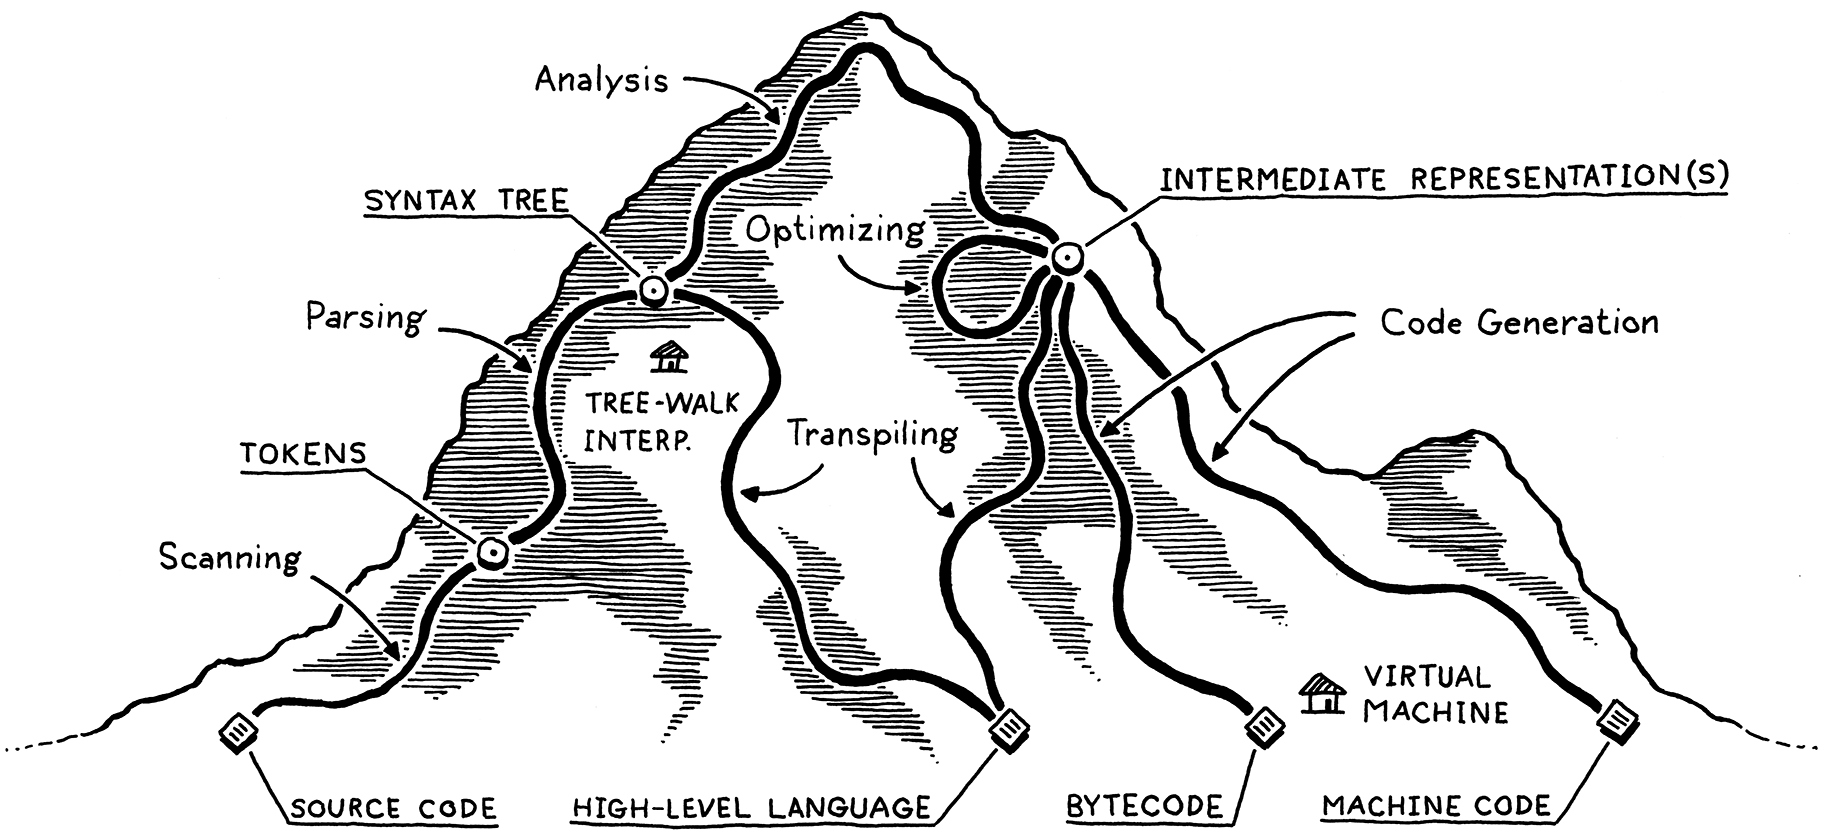
\includegraphics[width=0.8\textwidth]{mountain.png}
    \caption{Funktionsweise eines Interpreters ZITIEREN!!!}
    \label{fig:interpreter}
\end{figure}

Der erste Schritt ist die Lexikalische Analyse. Dabei wird der Quellcode in einzelne Tokens zerlegt. Ein Token ist dabei eine Zeichenkette die eine Bedeutung hat. Ein Token kann z.B. ein Schlüsselwort wie "if" oder "while" sein, eine Zahl oder eine Variable. Die Tokens werden dabei in einer Liste gespeichert und an den Parser weitergegeben.

Der Parser ist der nächste Schritt. Er nimmt die Liste von Tokens und baut daraus eine Datenstruktur auf. Diese Datenstruktur wird in der Literatur Syntax Baum (engl. Syntax Tree) oder Abtract Syntax Tree (AST) genannt. Ein AST ist eine Baumstruktur die den Quellcode repräsentiert. Die Knoten des Baums sind dabei die Operatoren und die Blätter sind die Operanden. Der Syntax Baum ist dabei eine abstrakte Repräsentation des Quellcodes und enthält keine Informationen über die Bedeutung der einzelnen Knoten. 

\doublelinebreak

Von hier aus gibt es nun verschiedenste Möglichkeiten wie der Syntax Baum weiter verarbeitet werden kann. Bei einem Compiler wird der Syntax Baum in eine Zwischensprache übersetzt und dann in Maschinencode. Bei einem Interpreter wird der Syntax Baum direkt ausgeführt. Es gibt aber auch noch andere Möglichkeiten. So kann der Syntax Baum z.B. in eine andere Sprache übersetzt werden oder in eine andere Form der Zwischensprache. Der Syntax Baum kann auch in eine andere Form der Zwischensprache übersetzt werden und dann von einem Interpreter ausgeführt werden. Es gibt also viele verschiedene Möglichkeiten wie ein Interpreter oder Compiler aufgebaut sein kann.

Bei modernen Interpretern gibt es z.B. das Konzept von Just-In-Time (JIT) Compilation. Dabei wird der Syntax Baum in eine Zwischensprache übersetzt und dann aber nicht direkt ausgeführt sondern in einem JIT Compiler in Maschinencode übersetzt. Dieser Maschinencode wird dann ausgeführt. Der Vorteil dieses Ansatzes ist, dass der JIT Compiler den Maschinencode optimieren kann und so die Ausführung beschleunigt werden kann. So arbeiten viele Interpreter intern trotzdem mit einem Compiler und Ausführung von Maschinencode.

Weiterer Erklärungsbedard besteht noch bei dem Begriff eines transformierenden Interpreters so wie er in dem Titel dieser Arbeit angekündigt wird. Im Rest der Arbeit soll eine Sprache entwickelt werden welche grundlegenden Regeln des Lambda Kalküls implementiert und so die Modellierung aller berechenbaren Funktionen ermöglicht. Dieser Interpreter soll Quellcode mit Lexikalischer Analyse und Parsing in einen Syntax Baum übersetzen, diesen Syntax Baum dann in eine Zwischenrepresentation (IR) übersetzen, Umformungen und berechungen durchführen und den Resultierenden AST dann wieder in die Ausgangssprache übersetzten. Der Interpreter soll also den Quellcode nicht komplett ausführen sondern nur in eine andere Form übersetzen. Damit handelt es sich nicht um einen traditionellen Interpreter sondern um ein System das eher einem Transpiler ähnelt - Transpiler übersetzen Programme von einer Sprache in eine andere. Der Begriff Interpreter soll hier aber trotzdem verwendet werden weil die Interaktion des Nutzers mit dem System eher der eines Interpreters als eines Transpilers ähnelt. hier werden tatsächlich berechnungen durchgeführt und es werden auch immer Teile des ASTs tatsächlich ausgewertet.

Daher wurde hier auch der unübliche Begriff eines transformierenden Interpreters gewählt, wobei das Transformieren für die Umformungen und Berechnungen steht die der Interpreter durchführt um dies Ausgabe zu erzeugen.

\section{Design und Implementierung des Interpreters}

Nachdem jetzt alle grundlegenden Konzepte betrachtet wurden, soll es jetzt um die Implementation des Interpreters gehen. 

\subsection{Beschreibung der Programmiersprache Lambo}

Das Ziel dieser Arbeit ist sich die Implementation des Lambda Kalküls in einer Programmiersprache zu betrachten und dabei die grundlegenden Regeln des Lambda Kalküls zu implementieren. Da die Sprache so also keine starken Anforderungen an einen praktischen nutzen für besonders performante Berechungen oder generell an eine nützliche Programmiersprache stellt, können andere Konzepte und Eigenschaften in den Vordergrund gestellt werden, die normalerweise nicht zu einer gängigen Programmiersprache gehöhren und auch die Implementation vereinfachen.

Das Ziel soll eine Website mit einem Code Editor sein in dem man Quellcode eingeben kann und dann die verschachtelten Lambda Terme schritt für Schritt umformen und reduzieren kann (TODO: Screenshot). Dieser Auswertungsmechanismus ermöglicht nicht nur eine Leehrreiche Interaktion, für das verständlich machen der Regeln des Lambda Kalküls, sondern vereinfacht auch die Implementation des Interpreters wie sich später zeigen wird.

Weil die zu entwickelnde Sprache in einem Online Editor verwendet werden soll und nur auf den grundlagen des Lambda Kalküls basiert soll sie auch einen Namen bekommen der diese Eigenschaften widerspiegelt:
Daher wir die zu entwickelnde Sprache im folgenden Lambo (angelehnt an Lambda Online) genannt.

Wie im Lambda Kalkül soll es in der Sprache Lambo nur Funktionen geben. 
Um allerdings mehrere Funktionen in einem Programm modelieren zu können wird zusätzlich auch ein Statement für die Wertezuweisung benötigt. Dafür soll in Lambo das Schlüsselwort "def" verwendet werden. Außerdem soll statt der herkömlichen Notation mit $\lambda$ und . die Notation mit runden Klammern und geschweiften Klammern verwendet werden, da diese Notation für einen Qellcode sorgt der populären Programmiersprachen wie z.B. Python ähnelt.
Eine erste Skizze der Syntax von Lambo hat also die folgende Strucktur:
\begin{align*}
    \text{\textless lambo-programm\textgreater} & ::= \text{\textless statement\textgreater}* \\
    \text{\textless statement\textgreater} & ::= \text{\textless definition\textgreater} \\
    \text{\textless definition\textgreater} & ::= \text{def} \; \text{\textless variable\textgreater} \; \text{\textless expression\textgreater}\\
    \text{\textless expression\textgreater} & ::= \text{\textless variable\textgreater} \; | \; \text{\textless abstraction\textgreater} \; | \; \text{\textless application\textgreater}\\
    \text{\textless variable\textgreater} & ::= \text{\textless letter\textgreater +} \\
    \text{\textless abstraction\textgreater} & ::= (\text{\textless variable\textgreater})\{\text{\textless lambda-term\textgreater}\}\\
    \text{\textless application\textgreater} & ::= \{\text{\textless lambda-term\textgreater} \; \text{\textless lambda-term\textgreater}\} \\
    \text{\textless letter\textgreater} & ::= a \; | \; b \; | \; c \; | \; ... \; | \; z | \; A \; | \; B \; | \; C \; | \; ... \; | \; Z | \; 0 \; | \; 1 \; | \; 2 \; | \; ... \; | \; 9
\end{align*}
Die BNF zeigt die grundlegende Strucktur für ein Lambo Programm. Ein Lambo Programm besteht aus beliebig vielen Statements. Ein Statement wiederum ist eine Definition die mit dem Schlüsselwort "def" beginnt und einer Variable einen Lambda Ausdruck zuweist. Ein Lambda Ausdruck wiederum ist wie gewohnt entweder eine Variable, eine Abstraktion oder eine Applikation wobei die Syntax für die Lambda Ausdrücke hier ein Bisschen anderes gewählt ist als für das Lambda Kalkül üblich. Um diese Syntax verständlicher zu machen folgen nun einige Beispiele für Lambo Programme. \\ \\
Eine einfache Identitätsfunktion wie $(\lambda x.x)$ kann in Lambo wie folgt aussehen:
\begin{lstlisting}
def ifunc (x) {
    x
}
\end{lstlisting}
In Lambo muss aber jeder Ausrduckt eine Definition sein deshalb wird der Lambda Ausdruch hier dem Symbol "ifunc" zugewiesen. Gleichermaßen lässt sich auch eine Variable in Lambo definieren:
\begin{lstlisting}
def a b
\end{lstlisting}
Hier wird die Variable b dem Symbol "a" zugewiesen. Für eine Applikation geht das ganze dann so:
\begin{lstlisting}
def app {
    a b
}
\end{lstlisting}
Wieder ist eine Definition nötig um den Lambda Ausdurck in Lambo darzustellen. Hier wird die Aplikation von a auf b dem Symbol "app" zugewiesen. Auch verschachtelte Funktionen sind mit dieser Definition der Syntax möglich:
\begin{lstlisting}
def someapp {
    (x) {
        x
    }
    a
}
\end{lstlisting}
Hier wird someapp die Applikation der Identitätsfunktion auf a zugewiesen. 
Da unsere Syntax bereits mehrere Funktionen in einem Programm ermöglicht, ist es auch der folgende Quellcode ein gültiges Lambo Programm:
\begin{lstlisting}
def a b
def c d
def e f
\end{lstlisting}
\doublelinebreak
Damit lässt sich bereits alles modelieren was an berechnbaren Fukntionen möglich ist. Allerdings ist die Syntax noch nicht ganz vollständig. Es fehlt noch die Möglichkeit Funktionen mit mehreren Parametern zu definieren. Dafür soll in Lambo die Syntax für Abstraktionen erweitert werden. Die erweiterte Syntax für Abstraktionen sieht dann wie folgt aus:
\begin{align*}
    \text{\textless abstraction\textgreater} & ::= (\text{\textless variable\textgreater}*)\{\text{\textless lambda-term\textgreater}\}\\
\end{align*}
Damit sind nun auch Funktionen mit mehreren Parametern möglich z.B.:
\begin{lstlisting}
def func (x y) {
    x
}
\end{lstlisting}
Das entspricht dann der Funktion $(\lambda x.\lambda y.x)$ im Lambda Kalkül. Und kann in Lambo auch mit einstelligen Funktionen umgesetzt werden:
\begin{lstlisting}
def func (x) {
    (y) {
        x
    }
}
\end{lstlisting}
Dieses Konzept wird auch Currying genannt und ist eine wichtige Eigenschaft von Lambo. Currying bedeutet, dass eine Funktion mit mehreren Parametern in mehrere Funktionen mit jeweils einem Parameter umgewandelt wird. Die Funktion $(\lambda x.\lambda y.x)$ wird also in Lambo zu $(\lambda x.(\lambda y.x))$ umgewandelt. Das hat den Vorteil, dass Funktionen mit mehreren Parametern in Lambo nicht anders behandelt werden müssen als Funktionen mit nur einem Parameter. Das vereinfacht die Implementation des Interpreters und ist auch ein Grund warum die Syntax von Lambo so gewählt wurde wie sie ist. Um eine ähliche Vereinfachung auch für die Applikationen zu erreichen, soll in Lambo auch die Syntax für Applikationen erweitert werden. Die erweiterte Syntax für Applikationen sieht dann wie folgt aus:
\begin{align*}
    \text{\textless application\textgreater} & ::= \{\text{\textless lambda-term\textgreater} \; \text{\textless lambda-term\textgreater}*\} \\
\end{align*}
Damit wird die linksassoziativ der Applikation auch in Lambo übernommen und ermöglicht es so eineige Klammern einzusparen. Statt
\begin{lstlisting}
def app {
    {{a b} c}
}
\end{lstlisting}
kann in Lambo also auch
\begin{lstlisting}
def app {
    a b c
}
\end{lstlisting}
geschrieben werden. Damit ist die Syntax von Lambo bis auf Quelltext-Kommentare (TODO: siehe Anhang) vollständig.

\subsection{Implementierung des Interpreters}

\captionsetup{labelformat=empty}
\lstset{
    language=Java,
    frame=single,
    breaklines=true,
    numbers=left,
    stepnumber=1,
    showstringspaces=false,
    tabsize=1,
    breaklines=true,
    breakatwhitespace=false,
    xleftmargin=.1\textwidth,
    xrightmargin=.1\textwidth
}

Wie auch bei der ersten Implementationen eines Interpreters aus dem Buch von Nystrom (TODO: CITE!), soll auch hier der Interpreter mit Java implementiert werden. So müssen schwierige Probleme wie die Speicherverwaltung nicht beachtet werden und das Lambda Kalkül steht im Fokus. Außerdem lässt sich für den Lambo Interpreter in Java später leicht mit vorhandenen Java Bibliotheken eine funktionstüchtige HTTP API umsetzen.

Im folgenden werden die einzelnen Komponenten des Interpreters vorgestellt und die Implementation erläutert. Dabei wird allerdings auf den vollständigen Quellcode verzichtet und nur vereinfachte Quelltext-Ausschnitte der wichtigsten Teile der Implementation vorgestellt. Unter den Codebeispielen werden die Zeilennummern der jeweiligen vollständigen Quelltext Datei angegeben die im Anhang zu finden sind.

\subsubsection{Lexer}

Zunächst muss der Quelltext mit einem Lexer in einzelne Tokens zerlegt werden. Dafür braucht es eine Klasse für die Tokens:
\begin{lstlisting}[caption={TODO: Referenz zu Anhang}, captionpos=b]
public class Token {
    public final TokenType type;
    public final String lexeme;
}
\end{lstlisting}
Ein Token hat dabei einen Typ und ein Lexeme welches den Inhalt des Tokens repräsentiert. Der Typ des Tokens wird dabei durch eine Enumeration definiert:
\begin{lstlisting}[caption={TODO: Referenz zu Anhang}, captionpos=b]
public enum TokenType {
    LEFT_PAREN, RIGHT_PAREN, LEFT_BRACE, RIGHT_BRACE, EQUAL,
    IDENTIFIER,
    DEF,
    EOF
}
\end{lstlisting}
Jeder Token in der Sprache Lambo lässt sich also genau einem Typ zuordnen. Ein Token kann dabei ein Sonderzeichen wie "(" oder ")" sein, ein Schlüsselwort wie "def" oder eine Variable. Die Variable wird dabei durch den Typ "IDENTIFIER" repräsentiert und das Lexeme der Variable ist dann der Name der Variable.
Mit diesem Grundgerüst lässt sich nun der Lexer implementieren.
\begin{lstlisting}[caption={TODO: Referenz zu Anhang}, captionpos=b]
public class Lexer{
    private final String source;
    private final List<Token> tokens;
    ...Hilfsvariablen wie aktuelle Position im Quelltext usw. 

    public Lexer(String source){
        this.source = source;
        this.tokens = new ArrayList<>();
    }

    public List<Token> scanTokens(){
        while(!isAtEnd()){
            scanToken();
        }
        tokens.add(new Token(TokenType.EOF, "", null, line));
        return tokens;
    }

    private void scanToken() throws LexingError{
        char c = advance();
        switch (c) {
            case '(': addToken(TokenType.LEFT_PAREN); break;
            case ')': addToken(TokenType.RIGHT_PAREN); break;
            case '{': addToken(TokenType.LEFT_BRACE); break;
            case '}': addToken(TokenType.RIGHT_BRACE); break;
            case '=': addToken(TokenType.EQUAL); break;
            case ' ': case '\r': case '\t': break;
            case '\n': line++; break;
            default:
                if (isAlphaNumeric(c)) {
                    identifierOrKeyword();
                }
                break;
        }
    }

    private void identifierOrKeyword() {
        while (isAlphaNumeric(peek())) advance();
        String text = source.substring(start, current);
        if (text == "def") {
            addToken(TokenType.DEF);
        } else {
            addToken(TokenType.IDENTIFIER);
        }
        addToken(type);
    }

    ...Hilfsmethoden wie addToken usw.
}
\end{lstlisting}
Zugunsten der Übersicht wurde hier sehr viel weggelassen aber die wichtigsten Teile der Implementation sind hier zu sehen. Der Lexer wird mit dem Quelltext initialisiert und kann dann mit der Methode "scanTokens" die Liste der Tokens zurückgeben. Die Methode "scanTokens" iteriert dabei über den Quelltext und ruft für jedes Zeichen die Methode "scanToken" auf. Die Methode "scanToken" entscheidet dann anhand des aktuellen Zeichens welcher Typ von Token vorliegt und fügt diesen der Liste der Tokens hinzu. Die Methode "identifierOrKeyword" wird dabei aufgerufen wenn ein alphanumerisches Zeichen gefunden wird und entscheidet dann ob es sich um ein Schlüsselwort oder eine Variable handelt. Die Methode "addToken" fügt dann den Token der Liste der Tokens hinzu. In dem Teilen die hier ausgelassen wurden wird sich dazu immer das aktuell gelesene Lexeme gemerkt damit dieses dann in der Methode addToken dem Token hinzugefügt werden kann.

So kann mit nur einem Durchlauf über den Quelltext (und ein Bischen vor und zurückgucken) eine Liste von Tokens erstellt werden die dann an den Parser weitergegeben werden kann.

\subsubsection{Parser}

Weiterhin angelehnt an das Buch von Nystrom (TODO: CITE!) soll auch hier ein rekursiver Parser verwendet werden. Der Parser nimmt dabei die Liste von Tokens und baut daraus einen Syntax Baum auf. Dafür braucht es zunächst Klassen für die Knoten des Syntax Baums. Wie diese aufgebaut sind soll kurz am Beispiel der Klassen für die Knoten von Abstraktionen, Applikationen und Variablen gezeigt werden:
\begin{lstlisting}[caption={TODO: Referenz zu Anhang}, captionpos=b]
    public abstract class LamboExpression {
        public static class Abstraction extends LamboExpression {
            private final Variable boundVariable;
            private final LamboExpression body;
            ...
        }
    
        public static class Application extends LamboExpression {
            private final LamboExpression left;
            private final LamboExpression right;
            ...
        }
    
        public static class Variable extends LamboExpression {
            private final Token token;
            ...
        }
    
        public abstract <R> R accept(Visitor<R> visitor);
    
        public interface Visitor<R>{
            R visit(Abstraction abstraction);
            R visit(Application application);
            R visit(Variable variable);
        }
    }
\end{lstlisting}
Um die Abhängigkeiten zwischen den verschiedenen Expression Typen und den Methoden die diese verabeiten müssen leicht zu entkoppeln bietet sich das "Visitor Pattern" an (TODO: CITE!). Die Klasse LamboExpression ist dabei die abstrakte Basisklasse für alle Knoten des Syntax Baums die zu einem Lambda Ausdruck gehöhren (d.h. nicht für Definitionen). Auf die gleiche Art müssen auch noch Klassen für die Knoten der Statements und des gesamten Syntax Baums erstellt werden. Diese Klassen sind aber nicht so wichtig für das Verständnis des Interpreters und werden deshalb hier nicht gezeigt.

Die Umwandelung von der Liste von Tokens in einen Syntax Baum wird dann genau anhand der Regeln der BNF durchgeführt:
\begin{lstlisting}[caption={TODO: Referenz zu Anhang}, captionpos=b]
public class Parser {
    private final List<Token> tokens;
    private int current = 0;

    public List<LamboExpression> parse(){
        List<LamboExpression> expressions = new ArrayList<>();
        while (!isAtEnd()) {
            LamboExpression expression = matchExpression();
            expressions.add(expression);
        }
        return expressions;
    }

    private LamboExpression matchExpression(){
        if(peek().getTokenType() == TokenType.IDENTIFIER){
            return matchVariable();
        }
        if(peek().getTokenType() == TokenType.LEFT_BRACE){
            return matchApplication();
        }
        if (peek().getTokenType() == TokenType.LEFT_PAREN){
            return matchAbstraction();
        }
        throw error(previous(), "Expected expression.");
    }

    private LamboExpression.Variable matchVariable(){
        if(match(TokenType.IDENTIFIER)){
            return new LamboExpression.Variable(previous());
        }
        throw error(peek(), "Expected lambda expression.");
    }

    private LamboExpression matchAbstraction(){
        consume(TokenType.LEFT_PAREN, "Expected '('.", previous());
        LamboExpression.Variable variable = matchVariable();
        consume(TokenType.RIGHT_PAREN, "Expected ')'.", previous());
        consume(TokenType.LEFT_BRACE, "Expected '{'.", previous());
        LamboExpression expression = matchExpression();
        consume(TokenType.RIGHT_BRACE, "Expected '}'.", previous());
        LamboExpression.Abstraction abstraction = new LamboExpression.Abstraction(variable, expression);;
        return abstraction;
    }

    private LamboExpression matchApplication(){
        consume(TokenType.LEFT_BRACE, "Expected '{'.", previous());
        LamboExpression left = matchExpression();
        LamboExpression right = matchExpression();
        LamboExpression.Application application = new LamboExpression.Application(left, right);
        consume(TokenType.RIGHT_BRACE, "Expected '}'.", previous());
        return application;
    }

    ...Hilfsmethoden wie match, consume, error usw.
}
\end{lstlisting}
Dieser unvollständigen Parser ohne Currying und ohne Definitionen, liest immer den nächsten Token und versucht dann eine der Regeln aus der BNF der Lambo Grammatik zu vervollständigen. Die Methode parse() iteriert dabei über die Liste der Tokens und ruft für jeden Token die Methode matchExpression() auf. Die Methode matchExpression() entscheidet dann anhand des aktuellen Tokens welche Regel aus der BNF angewendet werden muss und ruft dann die entsprechende Methode auf. Die Methode matchVariable() erzeugt dabei einen Knoten für eine Variable, die Methode matchAbstraction() erzeugt einen Knoten für eine Abstraktion und die Methode matchApplication() erzeugt einen Knoten für eine Applikation. Die Methode matchExpression() wird dabei rekursiv aufgerufen um auch verschachtelte Lambda Ausdrücke zu verarbeiten. Die Methode parse() gibt dann eine Liste von Lambda Ausdrücken zurück die dann an den Interpreter weitergegeben werden kann. Diese simplen rekursiven Vergleiche mit der BNF reichen aus um einen Syntax Baum aufzubauen der dann an den Interpreter weitergegeben werden kann. Für die ganze Sprache von Lambo fehlen hier aber natürlich noch die Regeln für die Definitionen und für das Currying. Diese können im Anhang nachgelesen werden (TODO: Referenz zu Anhang).

An diesem Punkt liegt nun ein Syntax Baum vor der alle Informationen enthält die für die Auswertung der Lambda Ausdrücke nötig sind. In einem herkömlichen Interpreter kann nun der Syntax Baum direkt ausgeführt werden indem mann Knoten des Baums rekursiv abarbeiten und entsprechen mit der Host-Sprache (hier Java) ausführt. Da Lambo aber ein, wie oben selbst definiert, transformierender Interpreter ist, soll der Syntax Baum nicht direkt ausgeführt werden sondern in eine andere Form übersetzt werden. Dafür braucht es zunächst eine Klasse für die Zwischenrepresentation (ZR):

\subsubsection{AST mit De-Bruijn-Indizes als Zwischenrepresentation}

Im Zusammenhang mit den Regeln des Lambda Kalküls wurde bereits die Notation mit De-Bruijn-Indizes vorgestellt die imense Vorteile bei der Substitution von Variablen bietet. Um diese Notation auch im Lambo Interpreter nutzbar zu machen muss der vorhandene Systax Baum in einen neuen Systax Baum mit De-Bruijn-Indizes übersetzt werden. Dafür wird wieder das Visitor Pattern verwendet um nun die Repräsentation für einen Sysntax Baum in der Zwischenrepresentation zu definieren:
\begin{lstlisting}[caption={TODO: Referenz zu Anhang}, captionpos=b]
public abstract class DeBruijnExpression {

    public static class Abstraction extends DeBruijnExpression{
        private final DeBruijnExpression body;
        private final String oldTokenLexeme;
    }

    public static class Application extends DeBruijnExpression{
        private final DeBruijnExpression left;
        private final DeBruijnExpression right;
    }

    public static class Variable extends DeBruijnExpression{
        private final String name;
    }

    public static class DeBruijnIndex extends DeBruijnExpression{
        private final int index;
    }

    public abstract <R> R accept(Visitor<R> visitor);

    public interface Visitor<R>{
        R visit(Abstraction abstraction);
        R visit(Application application);
        R visit(Variable variable);
        R visit(DeBruijnIndex deBruijnIndex);
    }
}
\end{lstlisting}
Ein AST in dieser ZR hat dabei fast die gleiche Strucktur wie der ursprüngliche AST nur dass hier alle gebundenen Variabeln durch entsprechende De-Bruijn-Indizes ersetzt werden. Alle ungebundenen Variablen in einem Lambda-Ausdruck behalten allerdings ihren Variablennamen. In dieser Hinsicht wird hier von der zuvor vorgestellten Notation abgewichen.
Hier beginnt dann auch die erste Kernaufgabe des Interpreters. Der Interpreter muss den vorhandenen AST in einen AST mit De-Bruijn-Indizes übersetzen. Dafür wird hier zum ersten mal das Visitor Interface implementiert:
\begin{lstlisting}[caption={TODO: Referenz zu Anhang}, captionpos=b]
public class DeBruijnTranslator implements LamboExpression.Visitor<DeBruijnExpression>{

    private DeBruijnEnvironment environment = new DeBruijnEnvironment(null);
    private final List<String> reservedVariables;
    private final LamboExpression input;

    public DeBruijnExpression translate() throws RuntimeError {
        return input.accept(this);
    }

    @Override
    public DeBruijnExpression visit(LamboExpression.Abstraction abstraction) throws RuntimeError{
        Token lambdaVar = abstraction.getBoundVariable().getToken();
        if(environment.contains(lambdaVar.getLexeme()) || reservedVariables.contains(lambdaVar.getLexeme())){
            throw new RuntimeError(lambdaVar.getLine(), String.format("Variable %s already defined in this scope", lambdaVar.getLexeme()));
        }
        environment = new DeBruijnEnvironment(environment);
        environment.define(lambdaVar.getLexeme());
        DeBruijnExpression body = abstraction.getBody().accept(this);
        environment = environment.getEnclosing();
        return new DeBruijnExpression.Abstraction(body, lambdaVar.getLexeme());
    }

    @Override
    public DeBruijnExpression visit(LamboExpression.Application application) throws RuntimeError {
        DeBruijnExpression left = application.getLeft().accept(this);
        DeBruijnExpression right = application.getRight().accept(this);
        return new DeBruijnExpression.Application(left, right);
    }

    @Override
    public DeBruijnExpression visit(LamboExpression.Variable variable) {
        if (environment.contains(variable.getToken().getLexeme())) {
            return new DeBruijnExpression.DeBruijnIndex(environment.getVariableIndex(variable.getToken().getLexeme()));
        }else {
            return new DeBruijnExpression.Variable(variable.getToken().getLexeme());
        }
    }
}
\end{lstlisting}
Das Visitor Pattern erlaubt es die rekursive Übersetzung des AST in einen AST mit De-Bruijn-Indizes sehr entkoppelt zu Programmieren. Für jeden Knoten in unserem Ausgangs-AST gibt es eine Methode die diesen Knoten in einen Knoten des Ziel-AST übersetzt. Wird dabei in einem Teil-Ausdruck ein weiterer Knoten gefunden der übersetzt werden muss, wird mit accept() dieser ebenfalls rekursiv übersetzt. Das Ergebnis ist eine DeBruijnExpression wie sie zuvor definiert wurde.

\subsubsection{Interpretieren der Zwischenrepresentation}

Genau wie diese Übersetzung werden auch alle möglichen anderen Umformungen und Berechnungen mit Hilfe des Visitor Interface implementiert. Die absolut wichtigste Umformung ist dabei die Substitution von Variablen. Nur hierfür wurde überhaupt der Aufwand betrieben den AST in einen AST mit De-Bruijn-Indizes zu übersetzen.
Hierfür wird nun ein weiterer Visitor implementiert der diesemal rekursiv den AST mit De-Bruijn-Indizes durchläuft und dabei die Substitution von Variablen durch weitere DeBruijnExpressions durchführt:

\begin{lstlisting}[caption={TODO: Referenz zu Anhang}, captionpos=b]
public class DeBruijnSubstitution implements DeBruijnExpression.Visitor<DeBruijnExpression>{

    private final DeBruijnExpression input;
    private final Map<String, DeBruijnExpression> substitutes;
    private int depth = 0;

    public DeBruijnExpression evaluate(){
        return input.accept(this);
    }

    @Override
    public DeBruijnExpression visit(DeBruijnExpression.Abstraction abstraction) {
        depth++;
        DeBruijnExpression.Abstraction result = new DeBruijnExpression.Abstraction(abstraction.getBody().accept(this), abstraction.getOldTokenLexeme());
        depth--;
        return result;
    }

    @Override
    public DeBruijnExpression visit(DeBruijnExpression.Application application) {
        DeBruijnExpression left = application.getLeft().accept(this);
        DeBruijnExpression right = application.getRight().accept(this);
        return new DeBruijnExpression.Application(left, right);
    }

    @Override
    public DeBruijnExpression visit(DeBruijnExpression.Variable variable) {
        if(substitutes.containsKey(variable.getName())){
            IncrementFreeDeBruijnIndices incrementor = new IncrementFreeDeBruijnIndices(depth, substitutes.get(variable.getName()));
            return incrementor.evaluate();
        }
        return new DeBruijnExpression.Variable(variable.getName());
    }

    public DeBruijnExpression visit(DeBruijnExpression.DeBruijnIndex deBruijnIndex) {
        return new DeBruijnExpression.DeBruijnIndex(deBruijnIndex.getIndex());
    }
}
\end{lstlisting}
Die Klasse DeBruijnSubstitution nimmt dabei einen AST mit De-Bruijn-Indizes und eine Map von Variablen zu DeBruijnExpressions und ersetzt dann alle Variablen im AST durch die entsprechenden DeBruijnExpressions. Dabei wird die Tiefe der Verschachtelung mitgezählt um die DeBruijnExpressions entsprechend zu inkrementieren. Die Klasse IncrementFreeDeBruijnIndices ist dabei eine weitere Klasse die mit Hilfe des Visitor Interface die eigentliche Inkrementierung durchführt (REF ANHANG). Aufbauend darauf können alle weiteren Funktionen mit Hilfe des Visitor Interface implementiert werden. Um hier nicht den Rahmen zu sprengen werden hier werden allerdings die rekursiven Implemtationen für die Beta-Reduktion und die Alpha-Konversion nicht gezeigt da die gerade implementierte DeBruijnSubstitution bereits die wichtigste dieser Umformungen ist. Die restlichen Klassen können im Anhang gefunen werden (TODO: Referenz zu Anhang).

\subsubsection{Zurück zum Quellcode}

Ohne den Quelltext für eine Implementation hier im feinsten Deteil darzustellen sollte es klar sein das mit dem gleichen Visitor Interface auch wieder eine Umformung in die ursprüngliche Lambo Syntax möglich ist. Dafür wurde für die Sprache die Klasse DeBruijnPrinter (REF ANHANG) implementiert die den AST mit De-Bruijn-Indizes rekursiv wieder in einen gültigen Quelltext der Sprache Lambo übersetzt. Dieser wird dann zurück an den Nutzer gegeben und schließt so den Kreis der Interkation. Der Nutzer kann nun Lambo Code an den Interpreter geben, verschiedene Umformungen durchführen und bekommt dann wieder Lambo Code zurück. Damit ist der ,,Transformierende Interpreter'' fertig implementiert.

\section{Evaluation und Ausblick}

\lstset
{
    frame=no,
    basicstyle=\footnotesize,
    numbers=left,
    stepnumber=1,
    showstringspaces=false,
    tabsize=1,
    breaklines=true,
    breakatwhitespace=false,
    xleftmargin=.3\textwidth
}

Die Sprache Lambo ist eine sehr eingeschränke Sprache. Es gibt keine Literale, keine boolsche Artimethik, keine Listen, keine Schleifen und keine Möglichkeit auf die Funktionen des Betriebsystems zuzugreifen. Dennoch ist es möglich alle berechenbaren Funktionen in Lambo zu implementieren. Das ist natürlich nicht sehr praktisch aber es zeigt das Lambo tatsächlich eine universelle Programmiersprache ist (solange der Speicher nicht ausgeht). 
Das wird schön sichtbar wenn man bekannte Konzepte wie z.B. die genannte boolsche Artimethik in Lambo implementiert.

\subsection{Boolschek Artimethik}

Um boolsche Artimethik in Lambo zu implementieren braucht es zunächst die Möglichkeit boolsche Werte zu repräsentieren. Da die Zeichenketten "true" und "false" allerdings nicht von der Sprache reserviert sind lassen sich diese einfach selbst definieren:
\begin{lstlisting}
def true (t f) {t}

def false (t f) {f}
\end{lstlisting}
Gibt man diese Definitionen in den Lambo Interpreter ein und führt dann Beta Reduktionen oder Substitutionen durch passiert erstmal garnichts. Die Parameter sind nicht gebunden und deshalb lassen sich diese ausdrücke also auch nicht weider vereinfachen oder ineinander einsetzen. Fügen wird noch eine Definition für die Konjunktion hinzu um das zu ändern:
\begin{lstlisting}
def and (a b) {a b false}
\end{lstlisting}
Die Konjunktion ist hier eine einfache Applikation die mit zwei Argumenten aufgerufen werden kann. Fügen wir jetzt noch einen Aufruf unserer "and"-Funktion zu unserem Programm hinzu können wird mit den ersten Berechnungen beginnen:
\begin{lstlisting}
def true (t f) {t}

def false (t f) {f}

def and (a b) {a b false}

def berechnung {
    and true false
}
\end{lstlisting}
Und tatsächlich: Führt man dieses Programm nun im Lambo aus, indem man den Compiler anweist mehrere Substitutionen und Beta Reduktionen durchzuführen erhält man das folgende Ergebnis:
\begin{lstlisting}
def true (t f) {t}

def false (t f) {f}

def and (a b) {a b false}

def berechnung false
\end{lstlisting}
Wunderbar! Die Konjunktion funktioniert wie erwartet. Fügen wir nun noch eine Definition für die Disjunktion hinzu:
\begin{lstlisting}
def or (a b) {a true b}
\end{lstlisting}
Und fügen wir noch einen Aufruf der Disjunktion zu unserem Programm hinzu:
\begin{lstlisting}
def true (t f) {t}
def false (t f) {f}
def and (a b) {a b false}
def or (a b) {a true b}

def berechnung {
    or {and true false} false
}
\end{lstlisting}
Und führen wir das Programm wieder aus:
\begin{lstlisting}
...
def berechnung true
\end{lstlisting}
Auch die Disjunktion funktioniert wie erwartet. Ab hier lässt sich beliebige lange Fortfahen um noch viele weitere Konzepte mit Lambo zu implementieren. Für mehr Beispiele kann dazu wieder im Anhang nachgelesen werden (TODO: Referenz zu Anhang).

\subsection{Limitierungen der Implementation}

Ganz zum Schluss soll noch kurz auf die Limitierungen von Lambo und des Lambo Interpreters eingeganen werden. Wo diese Sprache natürlich in der Theorie jede Berechenbare Funktion modelieren kann gibt es einige sehr starke Einschränkungen. 

Als erstes erwähnenswert ist die Tatsache das ein Programm in Lambo nicht im herkömlichen sinne gestartet wird und dann durchläuft. Betrachtet man alle möglichen Definitionen in Lambo so gibt es einige die man beliebig oft reduzieren kann ohne das je eine "stabile" Form ereicht wird. Manche Terme wachsen auch ins unendliche. Deshalb ist der Interpreter auch so konstruiert das der Nutzer immer nur eine Beta-Reduktion oder Substitution auf einmal durchführt. Eine einzelne Beta Reduktion terminiert nämlich immer und der Nutzer kann so selbst entscheiden wie weit er die Berechnung durchführen will. Das ist für diesen Zweck nicht schlimm da es bei Lambo hauptsächlich um die Veranschaulichung von Berechnungen geht und nicht um die Ausführung von Programmen, für eine praktische Programmiersprache wäre das aber natürlich ein sehr disqualifizierendes Problem.

Der Speicherverbrauch ist ein weiteres Problem, welches in Lambo nicht ganz schön gelöst ist. Eine einzelne natürliche Zahl kann in Lambo schon sehr viel Speicher verbrauchen, da diese ja mit verschachtelten Lambda Termen dargestellt werden muss und diese im Sysntax Baum ja immer gleich mehrere Knoten und damit Java Objecte belegen. Das ist natürlich nicht sehr effizient und könnte weiterführen auch gelöst werden wenn Lambo zum Beispiel um grundlegene Literalte und Artimethik erweitert werden würde.

Das Hauptziel einer funkionierenden kleinen Programmiersprache auf der basis des untypisierten Lambda Kalküls wurde aber erreicht und die Implementation des Interpreters ist auch sehr einfach und leicht verständlich. Das macht Lambo zu einem guten Beispiel für die Veranschaulichung der Regeln des Lambda Kalküls und der Implementation eines Interpreters im allgemeinen.


\printbibliography
\end{document}
